\documentclass[12pt]{article}
 
\usepackage[margin=1in]{geometry} 
\usepackage{amsmath,amsthm,amssymb}
\usepackage{wrapfig}

\usepackage{graphicx}
\graphicspath{ {./images/} }

\usepackage{natbib}
\bibliographystyle{apalike}

\usepackage{epigraph}
\setlength \epigraphwidth {\linewidth}
\setlength \epigraphrule {0pt}
\AtBeginDocument{\renewcommand {\epigraphflush}{center}}
\renewcommand {\sourceflush} {center}

\usepackage{hyperref}
 
\begin{document}

\title{The meter-barrier problem}
\author{Dino Bektesevic \\ 
Exoplanets - Final Project}
\maketitle


\epigraph{\centering The aerodynamic migration of small solids near the meter-size barrier imposes the most stringent timescale constraint on planet formation: $\approx$ 100 years. (This is rivaled only by thesis, job and grant deadlines!)}{\textit{Andrew N. Youdin \\ Les Houches lecture, 2008}}
\newpage

\section{Introduction}

The origins and creation of the Solar System has always been a topic of interest in Astronomy. In broad strokes it was long understood that stars, and therefore the planetary systems around them, must form from the collapse of gas clouds. It was, also, long imagined that in this collapse the existing particles from withing the cloud would have to coalesce to form ever larger bodies from sub-micron dust to gas giants - a growth spur spanning 12, or more, orders of magnitude. \citet{Armitage07} offers an overview of different phases of this growth (quoted verbatim):

\begin{itemize}
    \item Dust - small particles ranging from sub-micron to cm in scale. These particles are well-coupled to the gas, but there can be slow drift either vertically or radially. Growth occurs through physical collisions leading to agglomeration.
    \item "Rocks" - objects of meter scale. These particles have increasingly weak coupling to the gas, and so it can be useful to approximate their dynamics as being a combination of Keplerian orbits plus aerodynamic drag. Growth through this size regime is deduced to be rapid but the mechanism remains uncertain.
    \item Planetesimals - bodies of kilometer scale and above. Planetesimals are massive enough that their dynamics are largely decoupled from that of the gas. A population of bodies of this size is often considered as the initial condition for subsequent stage of planet formation, since the evolution of such a population is a well-posed N-body problem involving primarily purely gravitational forces (though for smaller planetesimals, questions regarding the bodies material strength can also be pertinent). In the classical scenario for planet formation we ignore dust and rocks once planetesimals have formed, but in fact aerodynamically assisted accretion of small bodies may play a substantial role in protoplanetary growth.  This is “pebble accretion”.
    \item Earth mass - planets or progenitors of the giant planet cores. Once growing planets reach masses of the order of that of Earth, they again become coupled to the gas disk, though this time via gravitational rather than aerodynamic interactions. For terrestrial planet formation it is possible that the formation of Earth mass bodies occurs after the gas disk has been dispersed (in which case this coupling is moot), but for growing giant planet cores it is inevitable that interaction will take place.
    \item Planetary cores - cores with  masses  of  the  order  of 10 earth masses.  At around this mass, there is a transition from a quasi-hydrostatic core + envelope structure to a regime of rapid gas accretion.
\end{itemize}

It is not hard to see how, especially when spanning such a large range of condition and processes, developing a model of planetary evolution remains a hard problem with many facets that still remain unsolved. Considerable theoretical progress on protoplanetary disks and accretion processes were made in the late 1960's and 1970's despite the fact that the observational constraints were almost solely derived from Solar System observations. Incredible technological progress made in the last two decades have since then reinvigorated the discussion by providing us with better observational constraints on the processes. Missions like Deep Impact, Rosetta, Hayabusa 2 have provided or, in the case of Hayabusa 2, are yet to provide us with better measurements of physical properties of Solar System rocks and planetesimals. Observatories like ALMA that are capable of direct imaging of the protoplanetary disks give clues to the composition, shape and dynamics of environments in which planets form in details not possible ever before. We should not exclude the ability of exoplanets, of which thousands have been detected so far, to provide us with constraints on the composition and dynamics of subsequent evolution of Earth mass (and greater) objects. 

In this report I will focus on the transition period from dust to rocks. Specifically, I will focus on describing the, currently still unsolved, meter-barrier problem. This focus will be divided into three parts: I) defining and describing what the meter barrier problem is (section blag), II) modeling the growth through collisions of dust particles where I hope to present the issues related with collisional agglomeration (section blahblah) and III) possible ways these issues can be avoided by adopting the streaming instability model.

\section{The Meter-Barrier problem.}

As already implied, protoplanetary disks consist mainly of gas and dust particles. In the classical picture the gas orbits around the central body partially supported by the gas pressure while the dust tends to orbit on Keplerian-like orbits. Because of this additional supporting force exerted by pressure, gas can orbit at a lower velocities compared to appropriate expected Keplerian orbit. Since dust orbits with larger velocity than gas at a given radius, the dust feels a headwind caused by the slower orbiting gas. The resulting drag force, dependent on the relative velocities of the gas and dust and the size of dust particles, causes a loss of angular momentum and an inward drift of the dust particles. It is well established (\cite{Weidenschilling77}, \cite{Armitage07}, \cite{ChiangYoudin10}) that for meter sized objects the drift timescale, the characteristic time in which the particle would travel its current distance to the star, are on the order of 100 years. Meanwhile, the disk ages are estimated to lie in the ranges of $10^4$ to $10^6$ \citep{Weidenschilling77} and the planet forming timescales are estimated to be much larger than the drift timescales. This implies that agglomeration through certain ranges of object sizes must be incredibly quick as such objects can not exist in the disk for long. This problem is referred to as the "meter-barrier" problem. 

\subsection{Dynamics of dust and gas}
\label{subsec:dynamics}

The original derivation, as made by \citet{Weidenschilling77}, is closely followed to derive the magnitude of the headwind experienced by the dust. Realizing that gas is additionally supported by pressure and is in hydrostatic equilibrium allows us to write the gas equation of motion:
\begin{equation}
    \label{eq:vecacc}
    \frac{GM_{sol}}{r^3}\vec{r} - \frac{1}{\rho_g}\nabla P_g - \Omega^2\times\vec{r} = 0
\end{equation}
where $-\frac{1}{\rho_g}\nabla P_g$ is the force due to gas pressure support and  $-\Omega\times\vec{r}$ the centripetal force, $\Omega$ being the angular frequency. In general for truly Keplerian, i.e. elliptical, orbits the angular frequency and radius vector are a function of time, or better to say function of orbital position. Assuming a circular orbit allows us to write $\Omega\times(\Omega\times r) = GM_{sol}/r^2 = v_K^2/r = g$ which simplifies the expression \ref{eq:vecacc}. Expressing the radial direction only:
\begin{align}
    \label{eq:radialacc}
    \frac{GM_{sol}}{r^2} - \frac{1}{\rho_g}\frac{dP_g}{dr} - \frac{v_K^2}{r} &= 0 \\
    g - \frac{1}{\rho_g}\frac{dP_g}{dr} - g_K &= 0
\end{align}

Defining residual gravity $\delta g \equiv g-g_K$ as the apparent gravitational acceleration with respect to that of an idealized circular Keplerian orbit nets us:
\begin{equation}
    \delta g = \frac{1}{\rho_g}\frac{dP_g}{dr}
\end{equation}

From the definition of the residual gravity we can also express the rotational velocity of the gas $v_g$ as:
\begin{align}
    \delta g &= g - g_K \\
    \delta g &= \frac{V^2_g}{r} - \frac{V^2_K}{r}
\end{align}
leading, if $\delta g / g \ll 1$, to:
\begin{equation}
    \label{eq:dvdg}
    \delta v \approx - \frac{\delta g}{2 g}v_K
\end{equation}
where $\delta v$ is the deviation of the gas velocity from the circular orbital velocity\footnote{See appendix A for comments}. This is an important connection as it encapsulates the main idea behind Weidenschilling's derivation. The gas can orbit at a lower velocity than the dust as its additionally supported by pressure. Dust "plows" through slower gas feeling a drag force proportional to $\delta v$. 

What follows is the second part of Weidenschilling's derivation where he formulates how drag force removes the angular momenta from the dust particles causing them to spiral inwards. We begin by stating the general expression for drag force: 
\begin{equation}
    F_D = \frac{1}{2} \rho_g v^2 C_D A  
\end{equation}
where $C_D$ is the dimensionless drag coefficient, $A$ the cross sectional area of dust particle and $v$ the relative velocity of the dust particle and gas. \citet{Weidenschilling77} continues  by decomposing the velocity vector into its constituent parts. The velocity vector of a dust particle can be written as a sum of its radial and transverse velocities $\vec{v_d} = v_{d, r} + v_{d, \phi}$. The transverse velocity is then expressed relative to the gas velocity $v_{d, \phi} = v_g + w$ where $w$ is the transverse velocity of the dust relative to the gas. Assuming gas has no radial velocity, which is not a bad approximation considering we assumed hydrostatic equilibrium at the beginning, the headwind experienced by the dust particle is just its radial velocity component $v_{d, r}$ (denoted $u$ in the paper). The total wind velocity felt by the dust particle is $v= (u^2+w^2)^{1/2}$. Balancing the forces in the radial direction gives us:
\begin{equation}
    \label{eq:forceeq1}
    \frac{(v_g + w)^2}{r} + \frac{F_D u}{mv} - g = 0
\end{equation}

A dust particle orbiting in a protoplanetary disk at some distance r will have a specific angular momentum $l=(v_g + w)r$\footnote{The change in symbol to $l$ from $h$ in the paper is to avoid disk scale height confusion.}. torque1, the change of the angular momentum with time, can then be written as: 
\begin{equation}
    \label{eq:torque1} 
    \frac{dl}{dt} = \frac{d}{dt} \left[ (v_g+w)r \right] = -r\frac{F_D w}{mv}
\end{equation}
where $\frac{F_D w}{v}$ is the transverse component of the drag force.

From this point onward, I depart from tracing \citet{Weidenschilling77} derivation as closely as so far for three reasons: I) at least a minimal discussion of drag equations and approximate disk models would be required both of which, while informative, would be lengthy, in my case quite poorly informed, and out of scope of this report, II) it is possible to derive the qualitative behaviour of dust without having to justify choice of values, or functional forms, for many of the parameters (temperature, density, pressure, drag force etc.) by parameterizing the expressions over dimensionless quantities already introduced and III) for the expressions derived in \citet{Weidenschilling77} to be easily usable would require us to pick a drag law, solve for the velocity components, calculate the Reynolds number and if the calculated Reynolds number was not consistent with the picked drag law repeat the procedure until a self-consistent solution was found. Instead, drawing on other sourced cited liberally throughout this report, I parameterized the equations in terms of stopping time and approximated a single scenario, namely the one where $u$ and $w$ are small compared to the Keplerian velocity $v_K$. In this way none of the conclusions made by \citet{Weidenschilling77} are skipped, but much of the required additional discussion, and difficulty in solving equations \ref{eq:forceeq1} and \ref{eq:torque1}, are avoided.

 We define, via dimensional analysis, the stopping time as the characteristic time required for any initial momentum to be lost solely due to friction caused by drag much like\citet{Weidenschilling77} does:
\begin{equation}
    t_{\mathrm{fric}} = -\frac{mv}{F_D} 
\end{equation}

It is quite common to express the stopping time in its nondimensional form: 
\begin{equation}
    \label{eq:nondimfric}
    \tau_{\mathrm{fric}} = t_{\mathrm{fric}}\Omega_K
\end{equation}

Rewriting equations \ref{eq:forceeq1} and \ref{eq:torque1} in terms of $t_{\mathrm{fric}}$ (note also that this is essentially the equivalent of \ref{eq:radialacc} with an substitution IT SHOULD BE, BUT SUBS IS HARD TO SEE?!) :
\begin{align}
    \label{eq:}
    \frac{(v_g+w)^2}{r} -& \frac{u}{t_{\mathrm{fric}}} - g = 0 \\
    \frac{dl}{dt} = -&r\frac{w}{t_{\mathrm{fric}}}
\end{align}

By using the expressions from equation \ref{eq:torque1} again, this can be written as a system of equations:
\begin{align}
    \label{eq:forceeq2}
    \frac{(v_g+w)^2}{r} - \frac{u}{t_{\mathrm{fric}}} - g &= 0 \\
    \label{eq:torque2}
    \frac{d}{dt}\left[(v_g+w)r\right] = -r\frac{w}{t_{\mathrm{fric}}}&
\end{align}

If we adopt the case when the total wind velocity felt by the particle $v$, $w$ and $u$ are all $\ll v_K$ we linearize the equations by ignoring all second order and mixed terms consisting of one or multiple small values. Starting with the $(v_g+w)^2$ we have:
$$ (v_g+w)^2 = v_g^2 + 2v_gw + w^2 \approx v_g^2 + 2v_gw $$
and for $\frac{dl}{dt}$, by stating $v_{d, \phi}=v_g+w \approx v_K$, keeping in mind that $v_K$ is also a function of radius, and applying the chain rule:
$$\frac{dl}{dt} = \frac{drv_{d, \phi}}{dt} = \frac{drv_{d, \phi}}{dr}\frac{dr}{dt} = \frac{drv_{d, \phi}}{dr}u \approx u\frac{drv_K}{dr} \approx \frac{1}{2}uv_K$$ 

There is one more dimensionless quantity we need to introduce in order to simplify the equations. The ratio of half of the force exerted by the pressure and the gravitational force (see appendix \ref{appendix:A} for motivation) denoted $\eta$ is given by the expression: 
\begin{equation}
   \label{eq:eta}
    \eta \equiv -\frac{1}{2} \frac{1}{\rho_g \Omega^2 r } \frac{dP_g}{dr}
\end{equation}

Even though expression is not very intuitive its definition arises naturally whenever components of equation \ref{eq:vecacc} are being written out. Especially in more detailed calculations that include back-reaction of collisions that accelerate the gas as well as slow down the dust, such as the one made by \citet{Nakagawa86}\footnote{A definitive must read as it details many complex solutions to the equations of motions ignored here.}. Using the definition \ref{eq:eta} we can rewrite equation \ref{eq:dvdg} as\footnote{See appendix \ref{appendix:B}}: 
\begin{align}
    \delta v &= - \eta v_K \\
    v_g &= (1-\eta)v_K
\end{align}

This allows us to make the following simplification in our linearization: 
$$v_g^2 = (1-\eta)^2v_K^2 \approx (1-2\eta)v_K^2 $$

Returning to equation \ref{eq:torque2} we write:
\begin{align}
    \frac{1}{2}uv_K &= -r\frac{w}{t_{\mathrm{fric}}} \\
    \label{eq:transversewindvel}
    w &= \frac{1}{2} \frac{t_{\mathrm{fric}} uv_K}{r}
\end{align}
and for equation \ref{eq:forceeq2}:
\begin{align}
    \frac{(v_g^2 +2v_gw)}{r} - \frac{u}{t_{\mathrm{fric}}} - g &= 0 \\
    g_K - \frac{(2v_gw)}{r}  - \frac{u}{t_{\mathrm{fric}}} - g &= 0 \\
    -\delta g - \frac{(2v_gw)}{r}  - \frac{u}{t_{\mathrm{fric}}} &= 0 \\
    \label{eq:linearizedEOM}
    -\eta \frac{v_K^2}{r} - \frac{(2v_gw)}{r}  - \frac{u}{t_{\mathrm{fric}}} &= 0 
\end{align}

Substituting the relative transverse wind velocity $w$ from equation \ref{eq:transversewindvel} into equation \ref{eq:linearizedEOM} and simplifying nets us:
\begin{equation}
   \label{eq:radialwindvel}
    \frac{v_r}{v_K} = \frac{-\eta}{ \frac{v_K}{r}t_{\mathrm{fric}} + \frac{r}{v_K}t_{\mathrm{fric}}^{-1}}
\end{equation}
and \textbf{finally} substituting in the definition for nondimensional stopping time, equation \ref{eq:nondimfric} into equations \ref{eq:transversewindvel} and \ref{eq:radialwindvel} and simplifying again:
\begin{align}
    \label{eq:nondimradialwindvel}
    u = -2\eta v_K \frac{\tau_{\mathrm{fric}}}{1 + \tau_{\mathrm{fric}}^2} \\
    \label{eq:nondimtransversewindvel}
    w = \eta v_K \frac{\tau_{\mathrm{fric}}^2}{1 + \tau_{\mathrm{fric}}^2}
\end{align}

We can quickly and easily verify that the linearized equations reproduce the qualitative behaviour expected from \cite{Weidenschilling77} by plotting the individual and total components of the relative wind velocities and comparing the figures. Qualitatively comparing figure \ref{fig:windvel} with figure 2 in \cite{Weidenschilling77} shows remarkable similarities indicating that the linearization procedure did not introduce any significantly different assumptions to the ones made in the paper.
\begin{figure}[htbp]
    \label{fig:windvel}
    \centering
    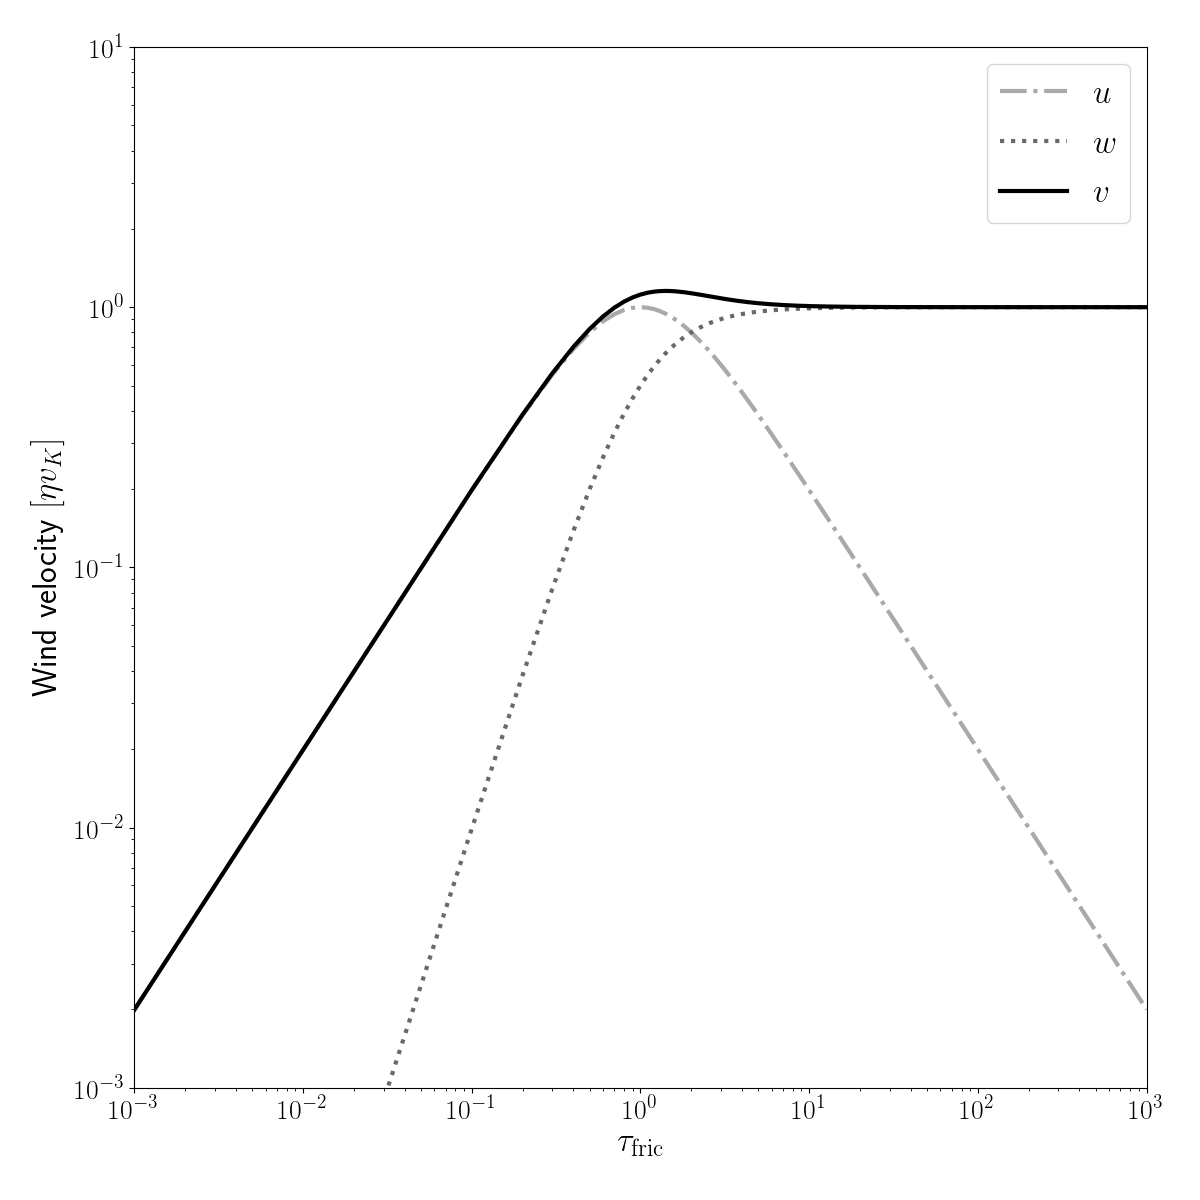
\includegraphics[width=0.5\linewidth]{windvel}
    \caption{The transverse and radial wind velocities, $w$ and $u$ respectively, alongside with the total wind velocity experienced by a dust particle in a protoplanetary disk are plotted in the units of $\eta v_K$ against the dimensionless stopping time $\tau_\mathrm{fric}$ }
\end{figure}

A quick derivation shows us that we expect the radial drift maximum to occur at $\tau=1$ meaning that the velocity with which the dust particle is moving in radial direction is at least on the order of $u=\eta v_K$. The value of $\eta$ depends on the selection of the protoplanetary model, as the model informs the functional form of the gas density $\rho_g$ (usually retrieved through a good fitting gas surface density expression) and pressure gradient $dP/dr$, but it is generally understood that for some local radius $r_0$ they are well approximated by a powerlaw: 
$$P = P_0 \left(\frac{r}{r_0}\right)^{-n}$$
where $n$ is generally picked to be positive, so that pressure, density etc. decrease outwards. Using such local powerlaw approximations and picking some numerical values it is possible to give an estimate of the magnitude of the radial wind velocity. \citet{Weidenschilling77} estimates a 100m/s for a 50cm large objects, \cite{Armitage07} and \cite{LesHouches} agree on a more conservative value of 60m/s and 56m/s respectively. As noted by all of them this implies decay times on the order 100-200 years. Figure \ref{fig:drifttimes}, taken from \cite{LesHouches} shows how in the interior, up to $\approx$ 10AU, meter sized objects consistently encounter almost the maximal radial wind velocities implying stopping time on the order of 50 to 10 000 years. This problem, previously explained qualitatively, where objects of certain sizes have incredibly characteristic life timescales  is the "meter-barrier" problem.
\begin{figure}[htbp]
    \label{fig:drifttimes}
    \centering
    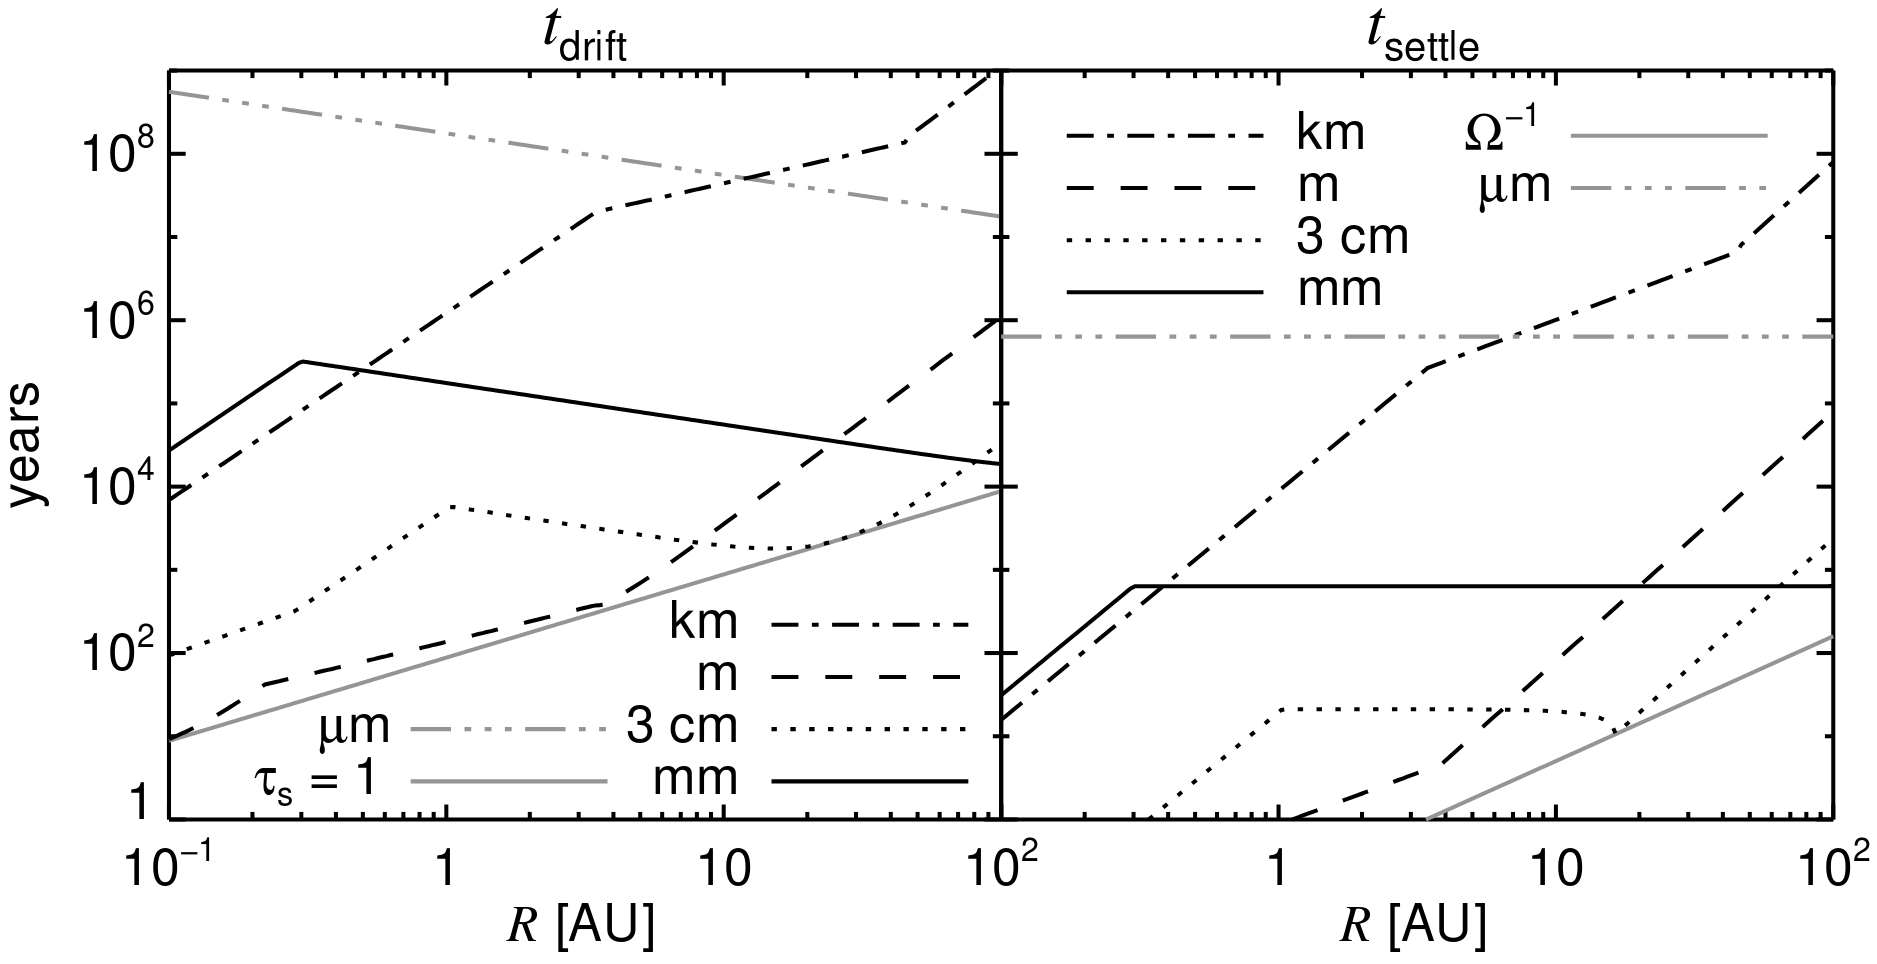
\includegraphics[width=0.8\linewidth]{drifttimesnotxt.png}
    \caption{(Left:) Particle radial drift timescale for several sizes vs. disk radius. The fastest migration at any radius is for a particle with $\tau_\mathrm{fric} = 1$ (grey curve). (Right:) Particle settling times, which are longer than the orbital time (grey curve), but shorter than the radial drift times.}
\end{figure}

\newpage
\section{Streaming instability}

\epigraph{\centering Since these collision speeds are comparable to a sand-blaster (credit to Eugene Chiang for this analogy) it is difficult to imagine net growth.}{\textit{Andrew N. Youdin \\ Les Houches lecture, 2008}}

Not every collision that occurs among dust and other objects necessarily produces an desirable outcome. Fragmentation, erosion, deflection ("bouncing"), cratering etc. are all negative outcome scenarios, i..e they do not produce growth. Although difficult to map out \cite{Windmark12} and \cite{Birnstiel2016} do so in an effort to map out how do collisional velocities and varying sizes of projectile and targets affect mass accretion onto an object. On figure \ref{fig:coloutcomes}, composed out of figures 8 and 6 from \citet{Windmark12}, \cite{Fulle} sketches out the collisional results as a function of colliding object sizes and the collisional velocities as expected from a, more detailed, model similar to the one presented in previous section. 
\begin{figure}[htbp]
    \label{fig:coloutcomes}
    \centering
    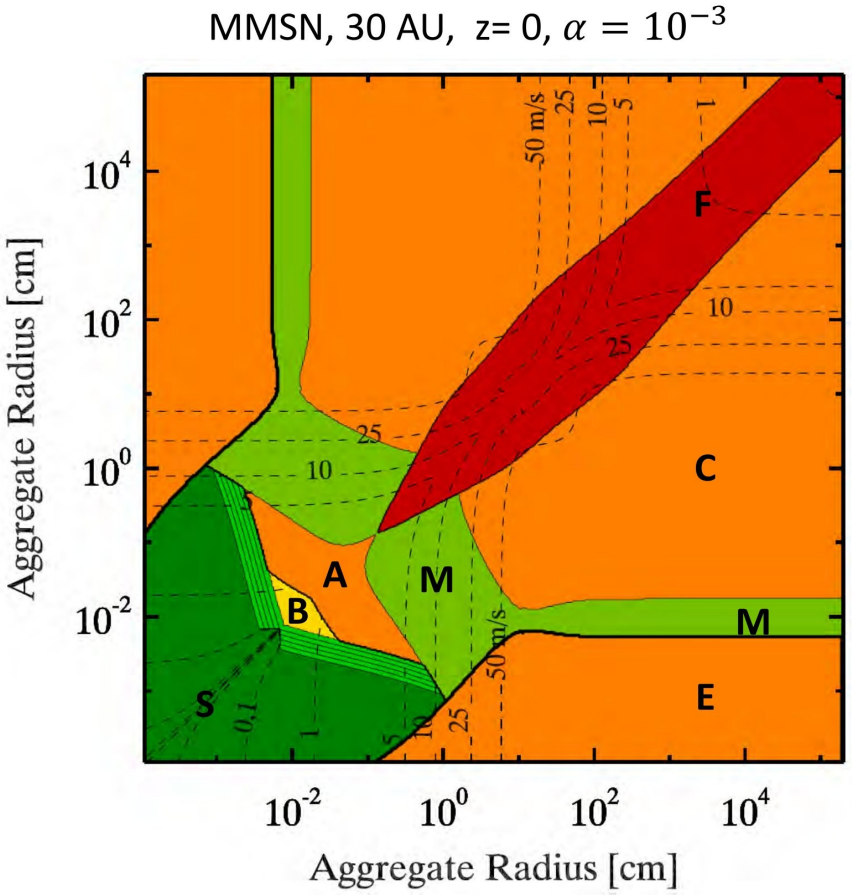
\includegraphics[width=0.5\linewidth]{FulleGraph.png}
    \caption{Average collisional outcome as a function of resulting particle sizes and collisional velocities. Green marks on average a net positive collisional outcome (sticking, agglomeration), while red and orange marks on average a net negative collisional outcomes (fragmentation). Yellow color denotes a netural event such as such as bouncing of mm-sized dust particles, a problem known as the "bouncing" barrier. Letters mark the expected type of processes (m-merger, b-bouncing, c-cratering, e-erosion, f-fragmentation). }
\end{figure}
What becomes apparent from the graph is that small particles, more tightly bound to the gas, grow quite easily, but once the particles cross a certain size the probability of them growing as a consequence of a collision is drastically reduced. A mechanism that would allow growing objects to skip or race through these barriers is required. 

Streaming instability is one such mechanism. As before, the idea of the system dynamics lies in the fact that gas orbits slower than dust, being partially supported by pressure. The dust particles feel a headwind in the opposite direction of their motion which causes them to lose angular momentum and spiral inwards. In section \ref{subsec:dynamics} we looked at the problem by ignoring the back reaction dust has on gas. This back reaction necessarily increases the gas velocity. If a local perturbation could cause a the particles to clump together more readily in some $dr$ around some $r$ (as in find themselves at those radii, not agglomerate) then the back reaction of dust particle collisions onto the gas would reduce the headwind felt by the dust there. In-spiraling dust from larger radii would encounter these bands of reduced headwind increasing the local density and further reducing radial drift, causing an exponential growth of initial clusters. Streaming instabilities were first described by \citet{Youdin05} led by an analogy with with the two stream instability in plasma physics. This process is also illustrated visually on figure \ref{fig:streaminginstabsim}, created from snapshots of a numerical simulation done by \cite{Simon16}.
\begin{figure}[htbp]
    \label{fig:streaminginstabsim}
    \centering
    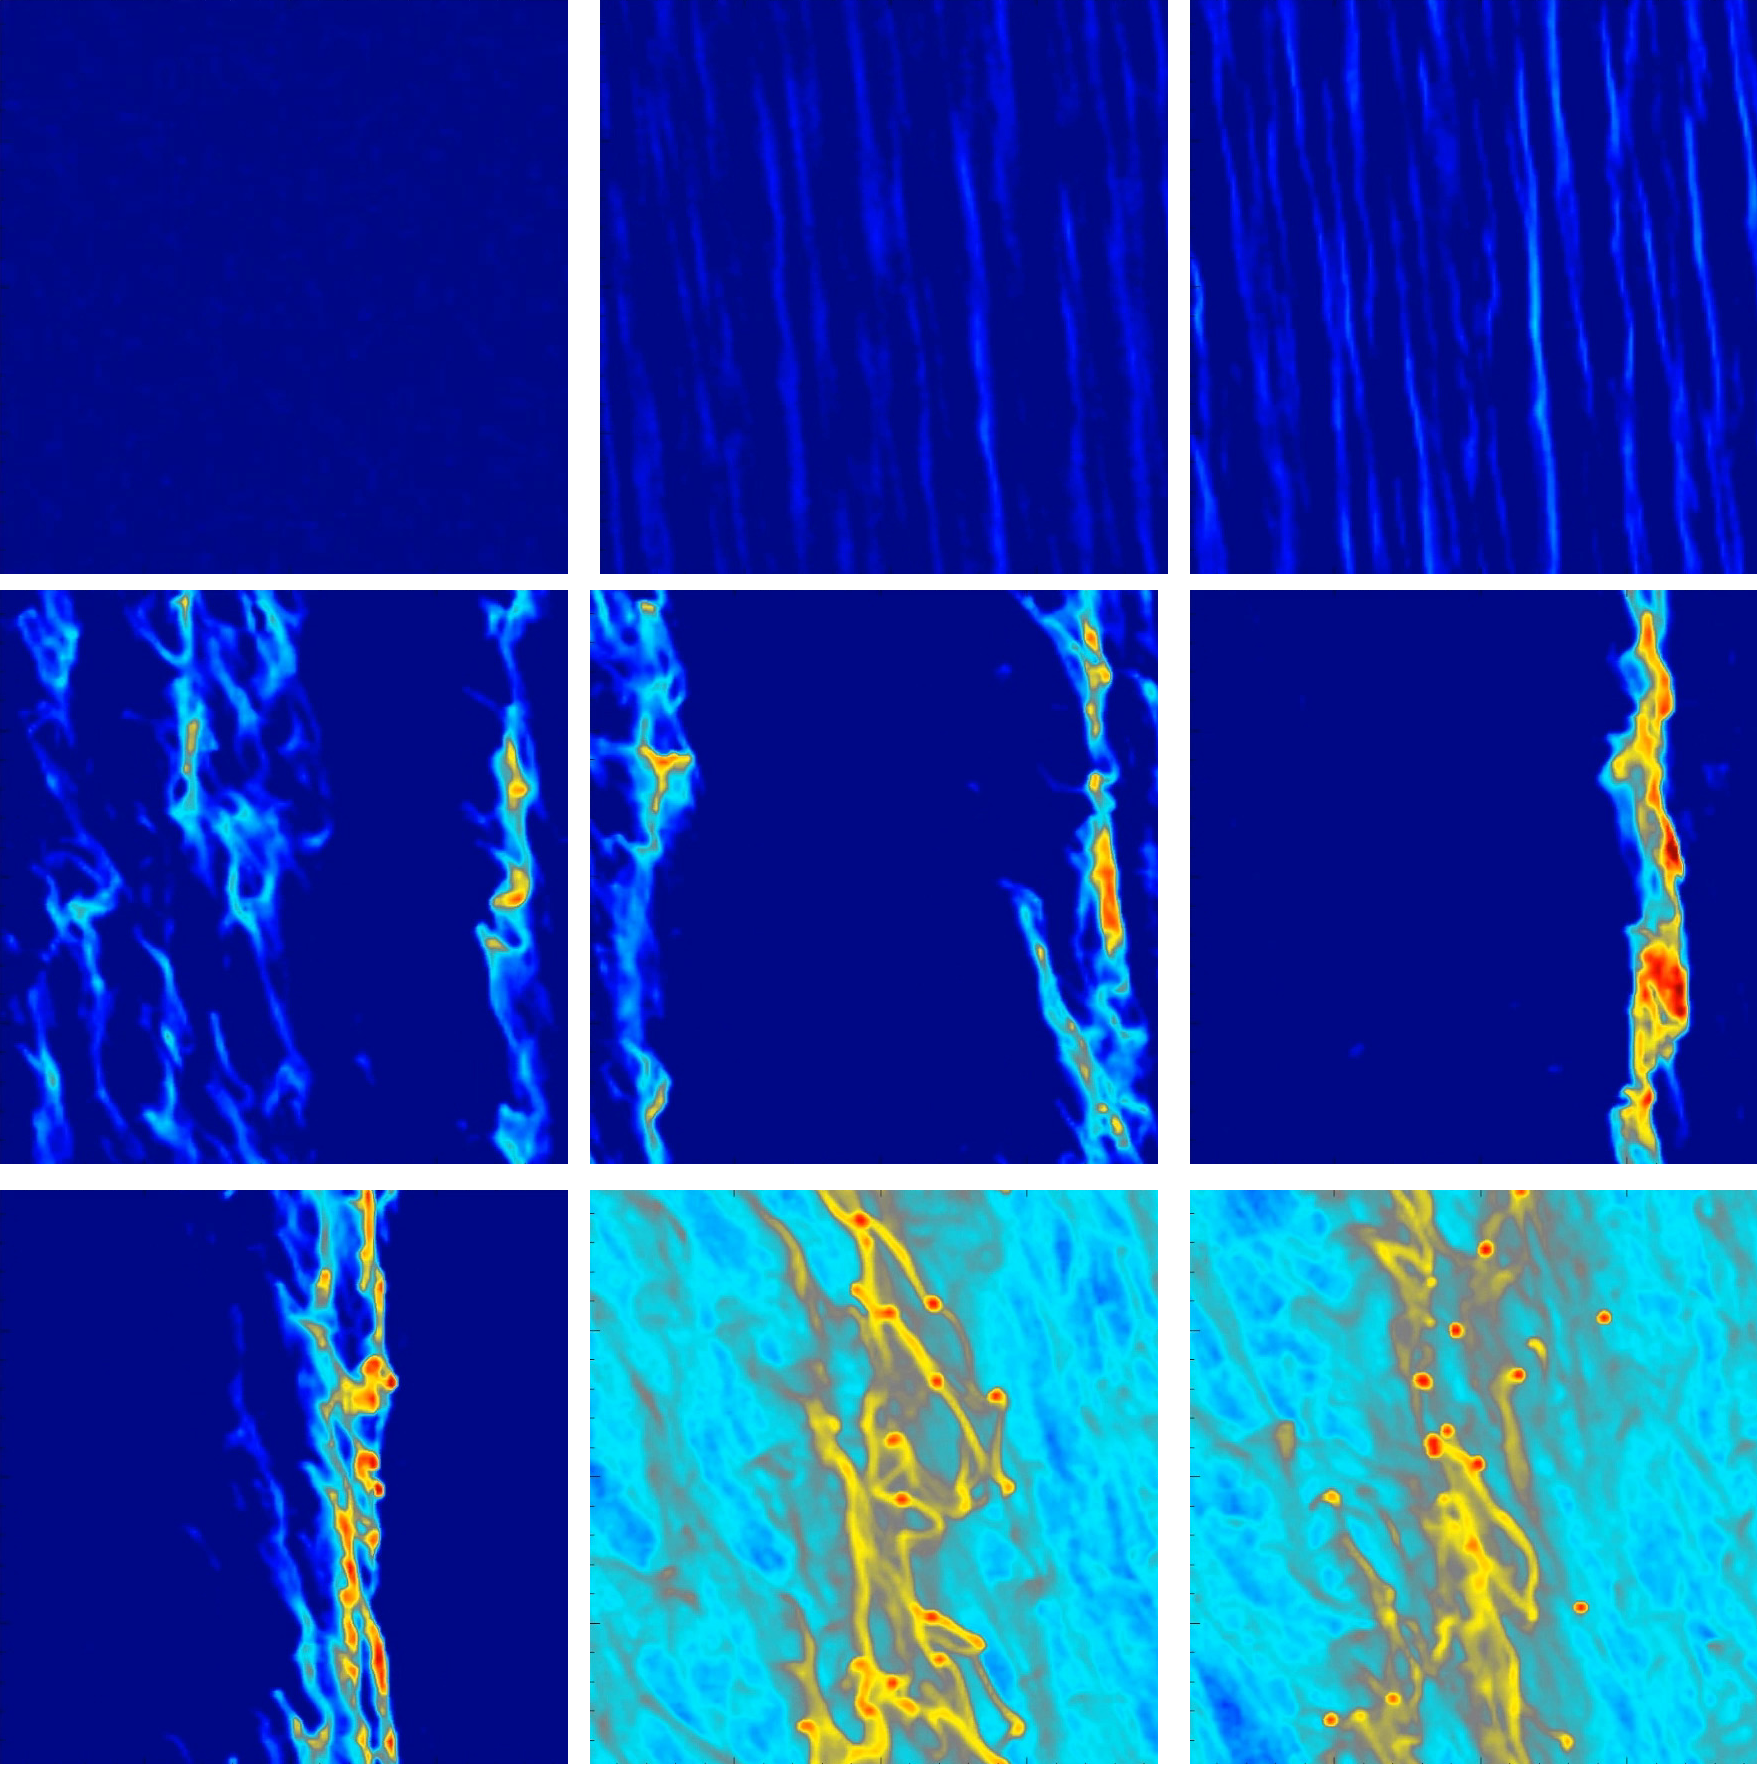
\includegraphics[width=0.55\linewidth]{images/streaminginstabsim.png}
    \caption{Numerical simulation of a streaming instability. The velocity gradient is top to bottom on the right hand side and bottom to top on the left (consider this in the reference frame of the rotating disk and you will see it's not a bad approximation since, as we saw, wind velocities can be on the order of $\ge 50$m/s). The color shows log of the ratio of surface density and the average surface density. First row shows how a small perturbation induces the creation of bands where the back reaction of dust-gas collisions reduces the apparent headwind. As particles stream inwards they clump into these bands increasing dust densities in them, second row. Third row depicts how at the moment when self gravity is turned on, the overdensities in the dust collapse to form planetesimals which then proceed to merge themselves (center, bottom right) thus quickly producing very large planetesimals 'out-of-the-box'.}
\end{figure}

\subsection{Modelling streaming instabilities}

Disk is modeled as two fluid Keplerian disk. One of the fluids is pressureless (dust) and the other incompressible (gas). Fluid motion is governed by Eulers equations:
\begin{align}
    \label{eq:eulerseq}
    \frac{d\rho}{dt} + \nabla \cdot (\rho v_d) &= 0 \\
    \nabla \cdot v_g &= 0
\end{align}
The equations of motion for the two fluids are given by Navier-Stokes equations for incompressible inviscid flow, changed to maintain notation in this report, are then:
\begin{align}
    \label{eq:navierstokesgas}
    \frac{d \vec{v_d}}{dt} + (\vec{v_d}\cdot \nabla)\vec{v_d} &= -\Omega^2r + \frac{\vec{v_d}-\vec{v_g}}{t_\mathrm{fric}}\\
    \label{eq:navierstokesdust}
    \frac{d \vec{v_g}}{dt} + (\vec{v_g}\cdot \nabla)\vec{v_g} &= -\Omega^2r + \frac{\rho_d}{\rho_g}\frac{\vec{v_d}-\vec{v_g}}{t_\mathrm{fric}} - \frac{1}{\rho_g } \nabla P
\end{align}

Notice the striking similarity between described in \ref{subsec:dynamics} and the expressions given by \cite{Youdin05}. If we follow through the same logic that arrived gave us equations \ref{eq:radialacc} and \ref{eq:forceeq2}, following in the footsteps of \cite{Nakagawa86}, but do not ignore the back reaction of collisions onto gas\footnote{The collisional contribution of gas onto dust is "hidden" in equation \ref{eq:forceeq1}. The back reaction onto gas should be equal and opposite to drag.} and write out the equations of motion for both gas and the dust we arrive at:
\begin{align}
    \frac{(v_g + w)^2}{r} &= -g + \frac{u}{t_\mathrm{fric}} \\
    \frac{GM_{sol}}{r^2}  &= - \frac{v_K}{r} + \frac{u}{t_\mathrm{fric}} - \frac{1}{\rho_g}\frac{dP_g}{dr} 
\end{align}
which are essentially only the radial component of the Navier-Stokes equations assuming a circular orbit and noting that velocities $u$ and $w$ represent the relative velocities of gas and dust. For full disclosure, I understand the expression is not really equivalent to the Navier-Stokes equations as a number of simplifications and assumptions were already made in deriving them that likely nullify the effects bore out by Navier-Stokes equations, namely the assumption of a steady state solution such that $d_tv_d = d_tv_g = 0$. This would be much more obvious if I adopted \cite{Nakagawa86} approach, where the equations of motion do not assume steady state as early as in \cite{Weidenschilling77}, but nevertheless the similarities are obvious and the point is that coupling of gas-to-dust must be treated with the same importance as dust-to-gas coupling, ironically showing how the mechanism that caused so much distress in section \ref{subsec:dynamics} is the same one providing a potential resolution in this one.  

The solution to equations \ref{eq:navierstokesgas} and \ref{eq:navierstokesdust} are sought via perturbative calculation around the steady state instead of linearization of a steady state. Considering the similarities between the equations of motions it is perhaps not surprising to see similarities between steps in the solution. 

\cite{Youdin05} begin by expressing the equations of motions in terms of the relative motions of the gas and the dust $\delta v$ and their center of mass motion $v = (\rho_dv_d+\rho_gv_g)/\rho$ where $\rho$ is the total density $\rho = \rho_d+\rho_g$:
\begin{align}
    \label{eq:comnavierstokesgas}
    \frac{d \vec{v}}{dt} + (\vec{v}\cdot \nabla)\vec{v} + F(\vec{\delta v}^2) 
    &= -\Omega^2r - \frac{1}{\rho_g } \nabla P \\
    \label{eq:comnavierstokesdust}
    \frac{d \vec{\delta v}}{dt} + (\vec{v}\cdot \nabla)\vec{\delta v} + (\vec{\delta v}\cdot \nabla)\vec{v} + G(\vec{\delta v})
    &= -\Omega^2r + \frac{\rho}{\rho_g}\frac{\vec{\delta v}}{t_\mathrm{fric}} + \frac{1}{\rho_g } \nabla P
\end{align}
where $F$ and $G$ are given by\footnote{Is equation \ref{eq:G} a typo in the paper?!}:
\begin{align}
    \label{eq:F}
     F(\vec{\delta v}^2) &\equiv \frac{1}{\rho_g } \nabla \cdot \left( \frac{\rho_g\rho_d}{\rho} \vec{\delta v} \vec{\delta v} \right) \\
    \label{eq:G}
     G(\vec{\delta v}^2) &\equiv \frac{\rho_g}{\rho}\vec{\delta v} \cdot \nabla\left( \frac{\rho_g}{\rho}\vec{\delta v} \right) - \frac{\rho_g}{\rho}\vec{\delta v} \cdot \nabla\left( \frac{\rho_g}{\rho}\vec{\delta v} \right) 
\end{align}
Note the discrepancy from section \ref{subsec:dynamics} definition of $v=(u^2+w^2)^{1/2}$. These slight differences can be subtle but important, for example $u$ previously marked what was essentially only the dust radial velocity $v_{d,r}$ as the gas had none, but in the perturbative approach the total radial headwind felt by a dust particle is its radial velocity $v_{d,r}$ added with the radial velocity of the gas $v_{g,r}$ and generally the average velocity of the inward migration of the dust $\overline{u_d}=\rho_g/\rho \overline{u}$ is matched by the outward migration of the gas $\overline{u_g}=\rho_d/\rho \overline{u}$. 
Also note that in \cite{Youdin05} the sign $\delta$ marks the perturbed quantities, as is custom, but I have so far been using them to mark differences $\Delta$. Because of the introduction of perturbations there arises a need to distinguish between a quantity and its perturbation, f.e. $V$ and $v$ corresponding to velocity and perturbation of the velocity around its $V$ value respectively. So far I tried to consistently express all equations in the same notation as the one I started with, but for elegance, readability and readers sake these notation changes have to be adopted from this point on.

In cylindrical coordinates $\vec{V} = U\hat r + W\hat\phi + Z\hat z$ and assuming thed steady state approximation $F=G=0$ we have:
\begin{align}
    \label{eq:steadystatestart}
    \overline{U} &= \overline{Z} = \overline{\Delta Z} = 0 \\
    \overline{W} &= \sqrt{ V_K^2 + \frac{r}{\rho}\frac{\partial P}{\partial r} } \approx \left( 1-\frac{\rho_g}{\rho}\eta\right)V_K \\
    \overline{\Delta U} &= -2 \frac{\rho_g}{\rho} \frac{\eta V_K\tau_\mathrm{fric}}{1 + \left(\frac{\tau_\mathrm{fric}\rho_g}{\rho}\right)^2 } \\
    \overline{\Delta W} &= \left(\frac{\rho_g}{\rho}\right)^2 \frac{\eta V_K\tau_\mathrm{fric}}{1 + \left(\frac{\tau_\mathrm{fric}\rho_g}{\rho}\right)^2 }
    \label{eq:steadystateend}
\end{align}
The perturbations of fluid quantities \ref{eq:steadystatestart}-\ref{eq:steadystateend} can be given in cartesian coordinates with respect to a center of mass of a small parcel of dust and gas, rotating around central object as $\Omega_0 = \overline{V_\phi}(r_0)/r_0$. The abscissa is then a translation $x=r-r_0$ and the ordinate evolves as $y=r_0(\phi-\Omega_0t)$. The benefit is that the differential rotation can be approximated as $\overline{W} = -q\Omega_0x\hat y$ where $q\approx 3/2$ for Keplerian orbits. 
\begin{align}
    \vec{V} &= -\frac{3}{2}\Omega_0x\hat{y} + \vec{v}(x,z,t) \\
    \vec{\Delta V} &= \overline{\Delta U}\hat x + \overline{\Delta W}\hat y + \Delta\vec{v}(x,z,t)\\
    \rho &= [1+\delta(x,z,t)]\rho_0 \\
    P &= \rho_0[-g_ex + h(x,z,t)]
\end{align}
where $g_e = \Delta g|_{r_0} = \frac{dP}{\rho_gdr}|_{r=r_0}$ locally experienced deviation from acceleration of a Keplerian orbit (i.e. "residual gravity as \cite{Weidenschilling77} puts it). Perturbations, as is custom, are taken to be plane waves: 
\begin{equation}
f(x,z,t) = fe^{i(k_xx + k_zz - \omega t)}
\end{equation}
where circular frequency is taken to be complex and the wavenumbers are real. The perturbations and steady state expressions need to be substituted into equations \ref{eq:comnavierstokesgas}-\ref{eq:G} (note that due to unfortunate change of notation capital letters now disappointingly replace lowercase ones) and simplified by dropping all zeroth and second order terms leaving only the first order perturbed quantities. I am not brave enough to perform this calculation so instead the perturbed equations are just copied from \cite{Youdin05}:
\begin{align}
    \label{eq:perturbstart}
    -i\omega\vec{v} -2\Omega v \hat x + \frac{\Omega}{2}u\hat y + \vec{F}' =& -i\vec{k}h - \delta g_e \hat x \\
    -i\omega\vec{\Delta v} - 2\Omega\Delta v \hat x + \frac{\Omega}{2}\Delta u\hat y + ik_x\Delta U \vec{v} + G' &= -\frac{\Delta \vec{v}+\delta \Delta\vec{V}}{f_gt_\mathrm{fric}} + i\vec{k}\frac{h}{f_g} \\
    -i\omega \delta + i\vec{k}\cdot\vec{v} &= 0 \\
    \vec{k}\cdot\vec{v} = f_d\vec{k}\cdot\vec{\Delta}& + f_gk_x\Delta U\delta
\end{align}
where $\vec{F'}$ and $\vec{G'}$:
\begin{align}
    \vec{F'} &= if_g\left[(f_p\vec{k}\cdot\Delta v + f_gk_x\Delta U\delta)\Delta V + f_dk_x\Delta U\Delta\vec{v}\right] \\ 
    \vec{G'} &= ik_x\Delta U\left[(f_g-f_p)\Delta\vec{v} - f_g\Delta\vec{V}\delta\right]
    \label{eq:perturbend}
\end{align}
where $f_g=\rho_g/\rho$ and $f_d=1-f_g$ are the gas and dust fractions. The above equations are related by a 6$^{\mathrm{th}}$ order dispersion relation describing how the wave and/or group frequency of the perturbation depend on its wavelength as it propagates through the disk. 

Since mathematics was abandoned perhaps I could give a qualitative explanation more focus. Taking the example of ocean waves, which is not a fair comparison as the perturbation in the disk cause a change in the mediums density but it is the only case of two different limits of dispersion relation (nondispersive and dispersive)  I could think of that still invokes desired mental imagery, we can discuss two scenarios: I) a large amplitude short wavelength wave and II) a small amplitude large wavelength wave, both in deep water. Such waves are described as a sum of many different wave components with different wavelengths. It is general knowledge that tsunamis are long wavelength waves of small amplitudes - meaning that if you were on a boat in the middle of an ocean you just might not be able to tell that a tsunami passed under you. It is also common knowledge that massive storms can occur in the middle of an ocean that produce incredibly large waves, but rarely do people near the shore panic over it. The physical reason behind that is that waves with large amplitudes but short wavelengths, compared to the depth, are dispersive systems. The wave components comprising that wave, sea waves are actually wave packets comprised of many waves of different wavelengths added together, that have different wavelengths travel at different velocities. So certain components of that wave race ahead while others lag behind and on the shoreline we see that whole wave arrive disassembledd' and do not perceive it as scary. However, in the case where the wavelength is large compared to the depth, we are dealing with a non-dispersive system. The components of that wave do not travel at different velocities and they all arrive at the same time, delivering large amount of energy to the shoreline at the same time. This, tsunamis, are therefore perceived as scary and people panic. The point of this\footnote{useless?} story is that it is the dispersion relation that informs us what kind of a system, dispersive or nondispersive, are we dealing with. The dispersion relation for sea waves in the dispersive case will give angular frequency $\omega(k)$ as an explicit function of wave-number (related to wavelength) $k$ while the nondispersive limit of that example will not $\omega\ne\omega(k)$. 
\begin{figure}[htbp]
    \label{fig:shortwave}
    \centering
    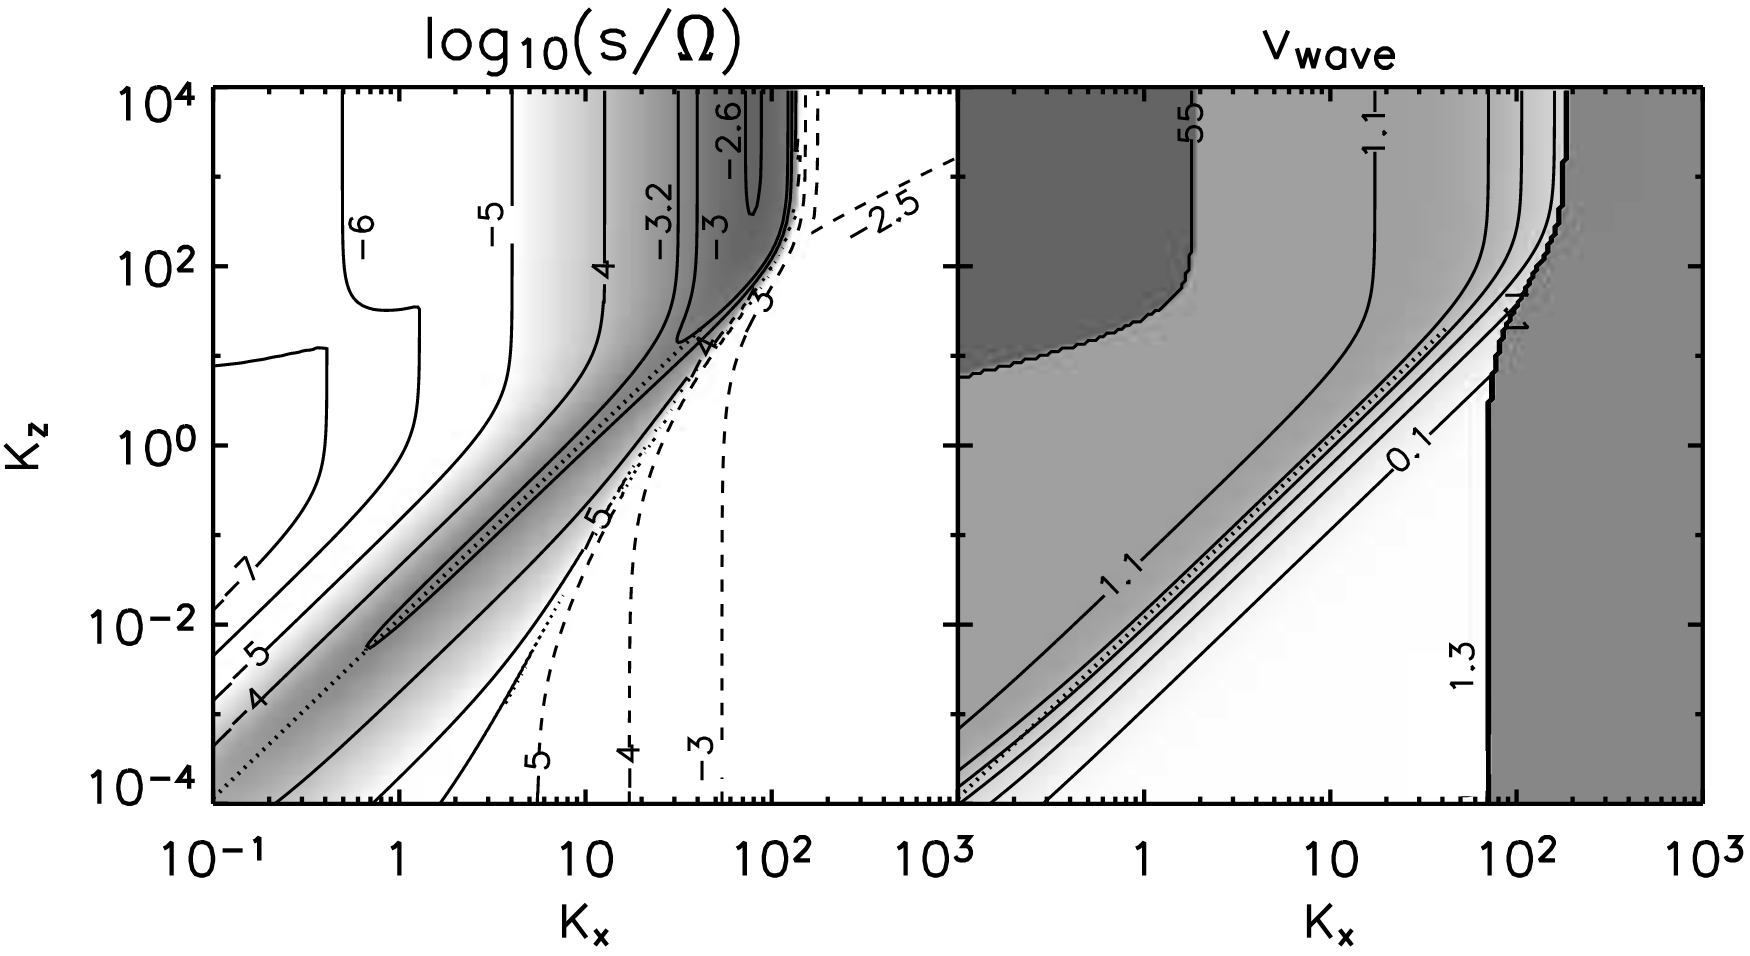
\includegraphics[width=0.7\linewidth]{images/shortwave.png}
    \caption{(Left:) Contours of groth rate, $\log_{10}(s/\Omega)$ (solid lines), and damping rate, $-\log_{10}(s/\Omega)$ (dashed lines), vs. $K_x$ and $K_z$. Two regions containing the fastest growing modes represent the short ($K_x\approx 80$, $K_z\ge100$) and long wavelength (diagonally $K_z\approx\tau_\mathrm{fric}K_x^2f_g^3$) regimes. (Right:) Wave speed $v_\mathrm{wave}=\omega_\mathbb{R}/k_x$ in units of $\eta v_K \tau_\mathrm{fric}$. Dark regions correspond to large phase speeds and damped weakly growing modes. }
\end{figure}

Coming back to the topic at hand, it is important to understand that the wave described by the equations \ref{eq:perturbstart}-\ref{eq:perturbend} is the perturbation and not directly the density or mass as in the sea wave example. However, we should not lose sight of the fact that this perturbation wave causes changes in pressure and velocity gradients, particle fractions etc. influencing where the dust is able to survive for longer and what radii/oribts are unfavorable. The dispersion relation for the two fluid disk are highly non-linear  6$^{\mathrm{th}}$ order equation that depends on the local density ratio $\rho/\rho$, orbital frequency $\Omega$, particle ($f_p$) and gas fraction $f_g$, wavenumber $k$, dimensionless stopping time $\tau_\mathrm{fric}$ etc. This makes its analysis a tad bit more complicated than the sea wave example, but not impossible. 

\cite{Youdin05} explore several different limits of the dispersion relation. short wavelength limit $K_z\gg K_x$, long wavelengths $K_z\lessapprox1$ $K_x\lessapprox1$ and the very long wavelengths $K_z\lessapprox\tau_\mathrm{fric}$. They find that the very long wavelengths are damped by frictional dissipation and quite uninteresting. In the short wavelength limit they find that dispersion relation that is independent of $K_z$. This mode is associated with the situation where radial pressure perturbations become negligible, which also logically makes sense\footnote{I'd argue that its surprising that the growth rate in this regime is only marginally faster than in the long wavelength case.}. Figure \ref{fig:shortwave}, taken from \cite{Youdin05}, shows this case quite clearly. Again, I have to restate that largest growth rates do not necessarily represent largest density increases, in fact \cite{Youdin05} find that the areas of largest density perturbations anti-correlate with the growth rate. 

\subsection{The real success of streaming instabilities.}
\begin{wrapfigure}{r}{0.4\textwidth}
  \begin{center}
    \label{fig:massradius}
    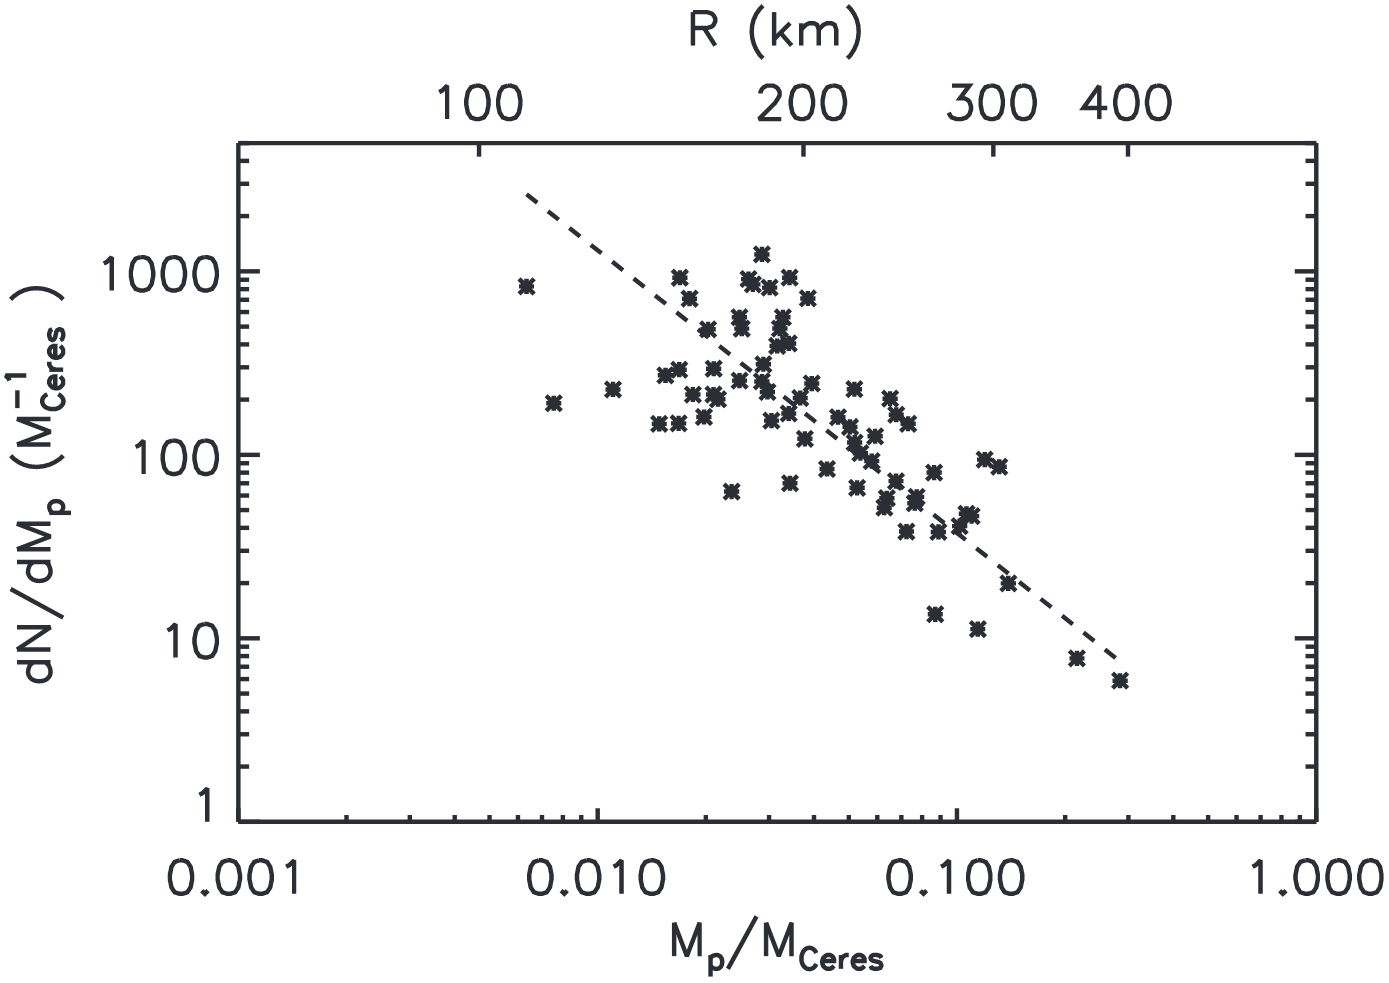
\includegraphics[width=0.39\textwidth]{images/diffmass.png}
  \end{center}
  \caption{Differential mass distribution functions for the fiducial simulation from \cite{Simon16}.}
\end{wrapfigure}

To see the real benefit of this approach we need to take a step back and refer back to the the simulation made by \cite{Simon16}. On figure \ref{fig:massradius}, taken from aforementioned paper, displayed are the planetesimal parameters as measured at the end of simulation. Notice how the simulation produce on the order of ten 400km sized objects with masses in the range 0.1-0.4 $M_\mathrm{Ceres}$ and thousands of 100-200 km sized objects in a model that is based on very firm physical reasoning
% required to break the wrapfig environment from reaching the next page
\noindent (remember that the derivation is based around perturbing a steady state solution of equations of motion known for decades, that include the backreaction of dust on gas). Self gravity is required only as a collapse mechanism that produces planetesimals since streaming instability induces local dust overdensities by itself. Streaming instability timescale is slower than disks dynamical (orbital) timescale but is faster than drift timescales which seems, to me, to correspond to observations. Instability does require, however, that the ratio of dust to gas be rather high, $\approx 1$, and that dust is moderately coupled to the gas such that inward drift of dust is significant. The latter seems to be well agreed upon in the community, but the requirement that dust to gas ratio is high is still widely discussed.


\newpage
\appendix

\section{Relating velocity deviation to residual gravity.}
\label{appendix:A}

This is not an obvious result and I am not sure how to recover it. The problem in recovering the expression lies foremost in the fact that there seems to be a better parameterization\footnote{On exact form of which nobody agrees either.} possible which has replaced this approach so this is not really visited again in another paper. What I believe was the procedure used by \citet{Weidenschilling77} is to derive the expression for uniform circular motion $v^2 = gr$:
\begin{align}
    \frac{d}{dr}v &= \frac{d}{dr}\sqrt{g(r)r} \\
    v' &= \frac{r g'(r) + g(r))}{2 sqrt(r g(r))} \\
    v' &= \frac{\sqrt{r} g'(r)}{2 \sqrt{g(r)}} + \frac{\sqrt{g(r)}}{2 \sqrt{r}} 
\end{align}
which, in the limit of small deviations and by approximating $g/r \ll 1$, becomes
\begin{align}
    \delta v &= \frac{\delta g}{2}\sqrt{\frac{r}{g}} + \frac{1}{2} \sqrt{\frac{g}{r}} \\
    \delta v &= \frac{\delta g}{2} \sqrt{\frac{r}{g}} = \frac{v_K}{g}\frac{\delta g}{2} \\
    \frac{\delta v }{v_K} &= \frac{\delta g}{2 g}
\end{align}

However, the exact reasoning is not crystal clear to me as the approximation $g/r \ll 1$ was never explicitly made by \citet{Weidenschilling77}, even though it is not baseless, who instead writes $\delta g/g \ll 1$ . \citet{LesHouches} does what is, perhaps, a more straightforward derivation of the link by defining the orbital velocity deviation in cylindrical coordinates as $\delta v_\phi \equiv v_\phi - v_K$ and by using the definition of circular velocity $v_K = \sqrt{GM_{sol}/r} = \Omega r$, to equate the pressure force, $-\frac{1}{\rho_g}\frac{dP_g}{dr}$, with the Coriolis force, $2\Omega\Delta v_\phi$:
\begin{align}
    \label{eq:simpledvdg}
    f_{Corr} + f_P &= 0 \\
    -\frac{1}{\rho_g}\frac{dP_g}{dr} + 2\Omega\delta v_\phi &= 0 \\
    \label{eq:etamotiv}
    \delta v_\phi = \frac{1}{2\rho_g\Omega}\frac{dP_g}{dr} &= \frac{1}{2\Omega}\delta g
\end{align}
which is the same result as the one recovered by \citet{Weidenschilling77} since by dimensional analysis we see that $\Omega = g/v_K$. Equation \ref{eq:etamotiv} is also providing us with a clear cut motivation for defining a new quantity $\eta$ as shown in equation \ref{eq:eta}.

\newpage
\section{Expressing velocity deviation to residual gravity over $\eta$}
\label{appendix:B}

Using the expression for circular Keplerian velocity $v_K = \Omega r$ and the definition of $\eta$ given by \ref{eq:eta} the relationship is immediately apparent from equation \ref{eq:simpledvdg}:
\begin{align}
    \delta v &= \frac{1}{2\Omega}\delta g \\
    \delta v &= -\frac{1}{2\Omega}\frac{1}{\rho_g}\frac{dP_g}{dr} \\
    \delta v &= -\frac{1}{2\Omega^2r}\frac{1}{\rho_g}\frac{dP_g}{dr} v_K \\
    \delta v &= - \eta v_K
\end{align}
from which it is also obvious that from the definition $\delta v = v-v_K$ follows
\begin{equation}
    v = (1-\eta)v_K
\end{equation}

Keeping the expression $g=\Omega^2 r$ in mind we can naturally, since they are equivalent, recover the same expression from \ref{eq:dvdg} as well: 
\begin{align}
    \delta v &= \frac{\delta g}{2 g} v_K \\
    \delta v &= \frac{\delta g}{2 \Omega^2 r} v_K \\
    \dots& \nonumber
\end{align}
where the remainder of the expressions are the same as above. This same relationship is also valid for $\delta g$. The difficulty in obtaining these expressions lies in the slightly different definitions of $\eta$: \cite{LesHouches} defines the pressure as $\frac{d\ln P}{2d\ln r}$, and later again as $\frac{dP}{2\rho_gV_K^2\ln r}$ \citep{Youdin05}, \cite{Armitage07} does not define it clearly but instead opts for the powerlaw approximation and then picks $P_0=nc_s^2$, where $c_s^2$ is the speed of sound, and I believe that the expression 1.10 for $\eta$ in \cite{Nakagawa86} is a typo and that $R\Omega^2$ should divide the expression instead. In hindsight all these expressions are equivalent when reverse-engineered from equation \ref{eq:eta} but connections are not as obvious in the 'forward' direction.

\newpage
\bibliography{references}

 
\end{document}